\section{Auswertung}
\label{sec:Auswertung}

% Messwerte: Alle gemessenen physikalischen Größen sind übersichtlich darzustellen.

% Auswertung:
% Berechnung der geforderten Endergebnisse
% mit allen Zwischenrechnungen und Fehlerformeln, sodass die Rechnung nachvollziehbar ist.
% Eine kurze Erläuterung der Rechnungen (z.B. verwendete Programme)
% Graphische Darstellung der Ergebnisse

\subsection{Aufname der Geiger-Müller Charakterisik}
\label{ssec:a1}

Die gemessenen Impulse $N$ sind in \autoref{tab:kennlinie} notiert.
Aus diesen Messwerten wird nun ein Plot erstellt, allerdings sind die Impulse mit der Unsicherheit $\sqrt{N}$ gemessen worden und werden für den Plot durch ihre Integerationszeit $\SI{60}{\second}$ geteilt.
Der zugehörige Plot ist dann in \autoref{fig:kennlinie} zu sehen.

\begin{figure}
    \centering
    \includegraphics[width=\textwidth]{build/plot_kennlinie.pdf}
    \caption{Plot der Geiger-Müller-Charakteristik}
    \label{fig:kennlinie}
\end{figure}

Wird das Ergebnis mit der Theorie verglichen, ist zu erkennen, dass hier ein Plateau dargestellt ist.
Von diesem wird nun die Steigung bestimmt.
Dafür wird eine lineare Ausgleichsgerade durch die Messwerte gelegt, die am ehesten in diesem Bereich liegen.
In diesem Fall wird das Plateau von $\SI{370}{\volt}$ bis $\SI{640}{\volt}$ angenommen.
Die Ausgleichsgerade besitzt dann die Form

\begin{equation}
    N = a \cdot U + b
\end{equation}

mit den Parametern

\begin{align}
    a &= \SI{0.019(4)}{\text{Imp}\per\volt\second}\\
    b &= \SI{160(2)}{\text{Imp}\per\second}.
\end{align}

Die Plateausteigung wird in $\%$ pro $\SI{100}{\volt}$ angegeben, das gelingt über die Umformung 

\begin{equation}
    a_\text{Plateau} = \frac{a \cdot 100 }{b}.
\end{equation}

Daraus ergibt sich dann das Ergebnis 

\begin{equation}
    a_\text{Plateau} = \SI{1.21(23)}{\%\per100\volt}.
\end{equation}

\subsection{Bestimmung der Totzeit}
\label{ssec:a2}

Aus den Messungen kriegen wir dann drei verschiedene Werte für $N$, einmal für die Quelle 1 und für Quelle 2 und für beide zusammen.
Es ergeben sich dann folgende Werte

\begin{align}
    N_1 &= \SI{96041(310)}{\text{Imp}\per120\second}\\
    N_{1+2} &= \SI{158479(398)}{\text{Imp}\per120\second}\\
    N_2 &= \SI{76518(277)}{\text{Imp}\per120\second}.
\end{align}

Aus der Theorie kann die Näherung \eqref{eq:tot2} verwendet werden, um die Totzeit $\tau$ zu berechnen.
Bevor die Werte eingesetzt werden, werden sie durch $120$ geteilt, um einen Wert pro Sekunde zu erhalten, es ergibt sich dann 

\begin{equation}
    \tau = \SI{115(4)}{\micro\second}.
\end{equation}

Eine andere Möglichkeit zur Bestimmung der Totzeit ist über ein Oszilloskop.
In \autoref{fig:oszillo} ist die Aufnahme dargestellt.

\begin{figure}
    \centering
    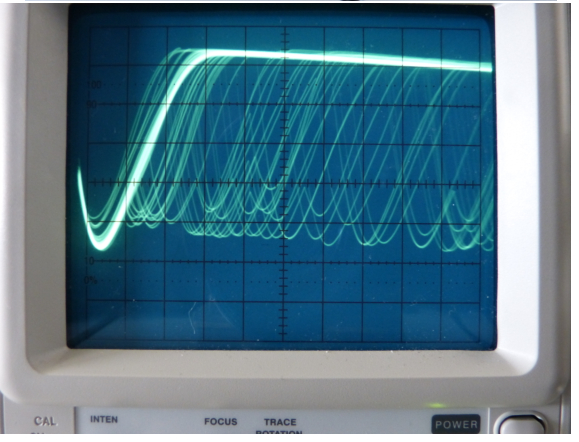
\includegraphics[width=\textwidth]{images/bild5.png}
    \caption{Momentaufnahme eines Oszilloskopbildes.}
    \label{fig:oszillo}
\end{figure}

Die Zeitachse ist auf $\SI{100}{\micro\second\per\text{DIV}}$ kalibriert.
Dann wird die Totzeit aus dem Bild als etwa 

\begin{equation}
    \tau = 100 \pm \SI{50}{\micro\second\per\text{DIV}}
\end{equation}

abgelesen.

\subsection{Bestimmung der Anzahl freigesetzten Ladungen pro Teilchen}
\label{ssec:a3}

Parallel zu der ersten Messung wurden die Stromstärken zu bestimmten Spannungen gemessen.
Diese Ergebnisse sind in \autoref{tab:stromstärke} notiert.

\begin{table}
    \centering
    \caption{Zählrohrstrom in Abhängigkeit der Spannung}
    \label{tab:stromstärke}
    \begin{tabular}{S[table-format=3.0] S[table-format=1.1]}
        \toprule
        \tableSI{U}{\volt} & \tableSI{I}{\micro\ampere} \\
        \midrule
        350& 0.3\\
        400& 0.4\\
        450& 0.7\\
        500& 0.8\\
        550& 1.0\\
        600& 1.3\\
        650& 1.4\\
        700& 1.8\\
        \bottomrule
    \end{tabular}
\end{table}

Mit \eqref{eq:z} kann aus $I$ und dem entsprechenden Wert für $N$ aus \autoref{tab:kennlinie} dann die Zahl Z berechnet werden, die Anzahl der freigesetzen Ladungen pro Teilchen.
Dann ergeben sich acht verschiedene Werte für Z, die ebenfalls geplottet werden.

\begin{table}
    \centering
    \caption{Zählrohrstrom in Abhängigkeit der Spannung}
    \label{tab:stromstärke}
    \begin{tabular}{S[table-format=1.1] S[table-format=1.2,table-figures-uncertainty = 1]}
        \toprule
        \tableSI{I}{\micro\ampere} & \tableSI{Z}{e^{16}} \\
        \midrule
        0.3 & 1.14+-0.19\\
        0.4 & 1.50+-0.19\\
        0.7 & 2.55+-0.18\\
        0.8 & 2.95+-0.19\\
        1.0 & 3.68+-0.19\\
        1.3 & 4.75+-0.19\\
        1.4 & 5.00+-0.18\\
        1.8 & 5.84+-0.17\\
        \bottomrule
    \end{tabular}
\end{table}

\begin{figure}
    \centering
    \includegraphics[width=\textwidth]{build/plot_zaehlstrom.pdf}
    \caption{Ergebnisse der Berechnung von $Z$}
    \label{fig:z}
\end{figure}